
%!TEX root = ../thesis.tex
%*******************************************************************************
%****************************** Third Chapter **********************************
%*******************************************************************************
\chapter{Reconstruction Framework Of SBND}
\label{ChapterReco}

% **************************** Define Graphics Path **************************
\ifpdf
    \graphicspath{{Chapter6/Figs/Raster/}{Chapter6/Figs/PDF/}{Chapter6/Figs/}}
\else
    \graphicspath{{Chapter6/Figs/Vector/}{Chapter6/Figs/}}
\fi

%********************************** %Opening  **************************************

The process of extracting physics quantities from the raw data recorded from an experiment is known as reconstruction.
At SBND, the physics characteristics of a particle can be reconstructed using multiple detection subsystems. 
For instance, a contained particle inside the TPC might deposit energy resulting in only waveforms recorded by the TPC wire planes and the PDS, meanwhile, an exiting particle might deposit additional energy in the CRT walls surrounding the TPC.
For a given particle, the TPC reconstruction can extract various quantities describing its topology, calorimetry and kinematics using charge information.
The PDS reconstruction can provide additional high resolution timing and calorimetry using light information.
The CRT reconstruction can indicate if the particle is fully contained inside the detector.
As a result, the reconstruction variables from all three detection subsystems are complementary to each other. 
%can be exploited for different analysis purposes such as cosmic rejection or particle identification.

This chapter provides a summary of the reconstruction framework at SBND.
Firstly, Sec. \ref{sec:reco_overview} gives an overview of the reconstruction workflow for each detection subsystem. 
The following Sec. \ref{sec:reco_tpc} includes the details of the TPC reconstruction workflow from start to end.
The reconstruction of the PDS and CRT subsystem are summarised in Sec. \ref{sec:reco_others}.
Descriptions of some high level analysis tools using the reconstruction variables collectively from each detection subsystem are included in Sec. \ref{sec:reco_ana_tools}.                 
Finally, the chapter is concluded in Sec. \ref{sec:reco_concluding_remarks} with some remarks.

%********************************** %First Section  **************************************

\section{Overview of The Reconstruction Framework}
\label{sec:reco_overview}

%Describe the overall workflow
Each detection subsystem in SBND requires a dedicated reconstruction workflow.
An overview is illustrated in Fig. \ref{fig:Reco_Workflow}.
The TPC reconstruction workflow is shown by the red boxes.
This process begins with raw wire waveforms going through the signal processing performed by the Wirecell tool kit \cite{wirecell}.
This is followed by a hit finding algorithm to identify hits on the waveform.
Output hits are then used by the Pandora package \cite{pandora} to produce a 3D-reconstructed interaction, denoted as a \textit{slice}.
The PDS reconstruction workflow also follows a similar process to the TPC, as shown by the blue boxes.
A waveform deconvolution is first performed on raw PDS waveforms to filter noise.
Then, a hit finding algorithm identifies optical hits on the waveform and reconstruction is performed on the hits.
The equivalent output to the TPC-reconstructed interaction from the PDS reconstruction is referred to as a \textit{flash}.
Finally, the reconstruction for the CRTs is much simpler compared to the other two subsystems, consisting of only a hit finding and a reconstruction algorithm, as shown by the orange boxes.
The reconstruction variables from each detection subsystem are produced independently and can be matched together if they originate from the same interaction. 
The variables can also be combined and input into different high level analysis tools to extract more complex properties of the underlying interaction. 

\begin{figure}[htbp!] 
\centering    
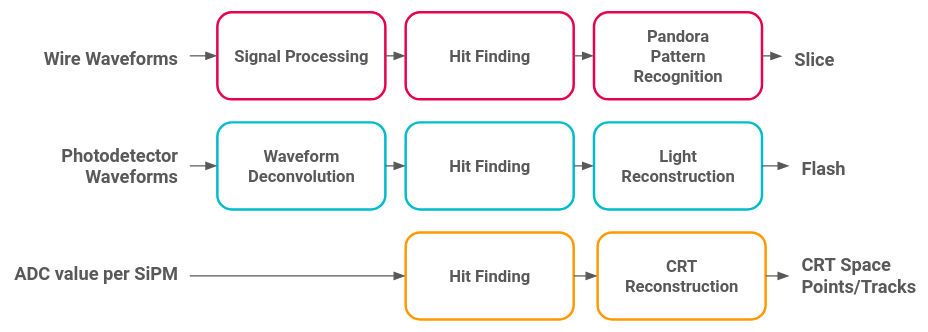
\includegraphics[width=1.0\textwidth]{Reco_Workflow}
\caption[Reconstruction Framework of SBND]{
Overview of the reconstruction workflow of the SBND detector.
}
\label{fig:Reco_Workflow}
\end{figure}

\section{Time Projection Chamber Reconstruction}
\label{sec:reco_tpc}

This section covers the TPC reconstruction workflow, starting with Sec. \ref{sec:signal_process} on the signal processing.
Sec. \ref{sec:hit_find} and \ref{sec:pandora} then detail the hit finding and Pandora reconstruction.
Finally, Sec. \ref{sec:trkshwbdt} delves into the track and shower separation algorithm of Pandora. 

\subsection{Signal Processing}
\label{sec:signal_process}

%Signal Processing
Signal processing is the first crucial step of TPC reconstruction, which is to deconvolve digitised raw waveforms and account for detector effects such as noise, electronics response and field response. 
At SBND, signal processing is implemented using the WireCell tool kit \cite{wirecell}.
The tool has been used by other LArTPC experiments such as MicroBooNE \cite{wirecell} and ProtoDUNE \cite{wirecell_protodune}.
%Both implementations here have demonstrated excellent performance to acquire deconvolved charge by performing deconvolution in time and wire dimension over the traditional deconvolution in time dimension only. 

Fig. \ref{fig:signal_processing_steps} shows an illustration of the signal processing steps.  
In grey is the \textit{true} ionisation charge deposited on a wire, simulated without any detector effects applied.
In red is the raw waveform resulting from the deposited charge, convolved with noise, electronics and field response.
The first step is noise filtering to remove the excess and correlated noise from raw waveforms.
Then, the measured charge is deconvolved from the electronics and field response to recover the original charge deposited on the wire, as shown in orange.
The deconvolution is 2D, where response functions consider the time response of a single wire as well as of neighbouring wires.
This step is particularly important for the induction planes to convert bipolar into unipolar signals, such that the integral of the waveform can be used for charge estimation.

High frequency filters are applied to attenuate noise that is artificially amplified, using Gaussian and/or Weiner filters depending on whether the signal is unipolar or bipolar.
The example here is a bipolar waveform and therefore, has both Gaussian and Weiner filters applied, shown in yellow and green respectively.
Then, low frequency filters are utilised for peak finding and local baseline removal, as shown in blue.
Finally, the deconvolved waveform per wire after baseline removal is shown in purple, which closely resembles the true charge as shown in grey.
This demonstrates the excellent performance of the signal processing chain to de-tangle detector effects from raw waveforms and recover the original deposited charge.  

Fig. \ref{fig:signal_processing_waveform} depicts event displays of a simulated neutrino event as seen by wires on the u plane.
The left figure depicts distributions of true charge deposition on wires (shown in grey in Fig. \ref{fig:signal_processing_steps}).
The middle and right figures illustrate the charge distributions using raw waveforms before signal processing (shown in red in Fig. \ref{fig:signal_processing_steps}) and deconvolved waveforms after signal processing (shown in purple in Fig. \ref{fig:signal_processing_steps}).
The right figure shows clearly two tracks and two showers, that closely resemble the true charge deposition shown in the left figure, demonstrating the performance of signal processing.
It is noted that the signal processing chain in SBND is currently a work in progress, as labelled so in Fig. \ref{fig:signal_processing_steps} and \ref{fig:signal_processing_waveform}.
At the time of writing, work on the optimisation of the chain specifically for SBND electronics has begun.

\begin{figure}[ht!] 
\centering    
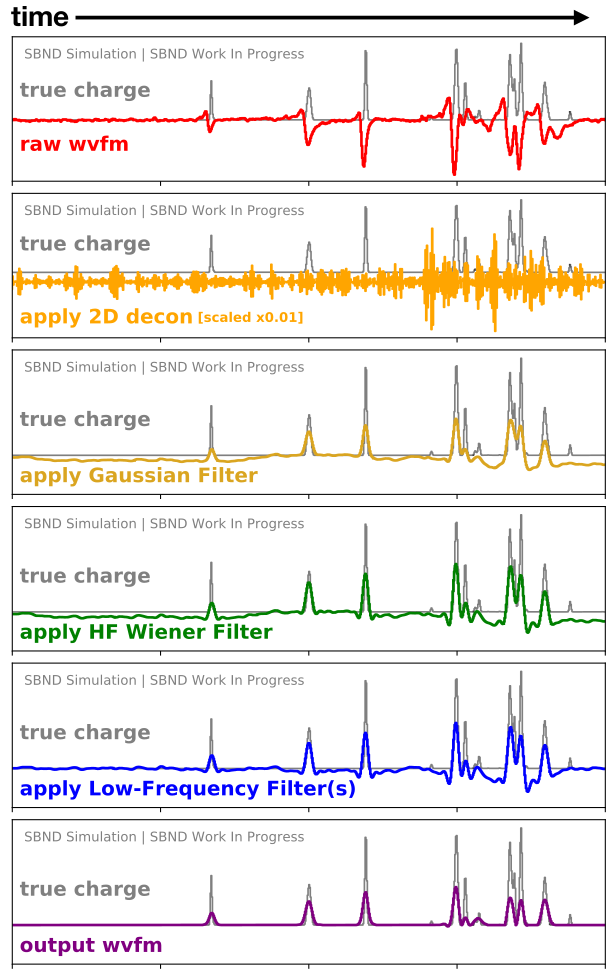
\includegraphics[width=0.45\textwidth]{signal_processing_steps}
\caption[Signal Processing Steps]{
Steps of signal processing applied to a bipolar raw waveform \cite{LynnSignal}.
}
\label{fig:signal_processing_steps}
%\end{figure}
%\begin{figure}[htbp!]
\vspace{0.5cm}
\centering    
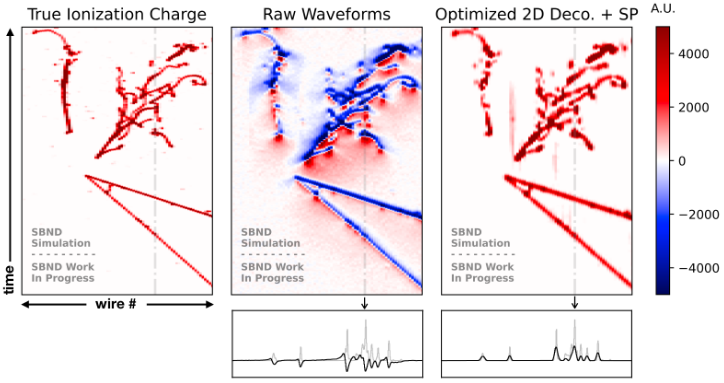
\includegraphics[width=0.85\textwidth]{signal_processing_waveform}
\caption[Event Displays of a Neutrino Interaction Before and After Signal Processing]{
Event displays of a simulated neutrino event using true ionisation charges (left), raw waveforms (middle) and deconvolved waveforms (right) \cite{LynnSignal}.
}
\label{fig:signal_processing_waveform}
\end{figure}

\subsection{Hit Finding}
\label{sec:hit_find}

After signal processing, hit finding is performed on deconvolved waveforms to search for Gaussian-shaped pulses above a threshold.
This is done using the \texttt{GausHitFinder} module \cite{gaushitfinder} by fitting a series of Gaussians to the waveform.         
The number of pulses is determined by the number of maxima found when differentiating the waveform, where each pulse represents a hit. 
Fig. \ref{fig:gaushit} demonstrates the hit finding process for a deconvolved waveform, showing four hits have been identified and fitted with a Gaussian.
Once the hits are fitted, information describing the hit is extracted and used by downstream reconstruction.
The peak time represents the time at which the charge arrives at the wire, used for determining the drift position and matching hit coincidence across wire planes.
The height and the width of the Gaussian are used to calculate the integral of the pulse, representing the deposited charge on the wire, subsequently used in downstream analysis for calorimetry computation.

\begin{figure}[htbp!] 
\centering    
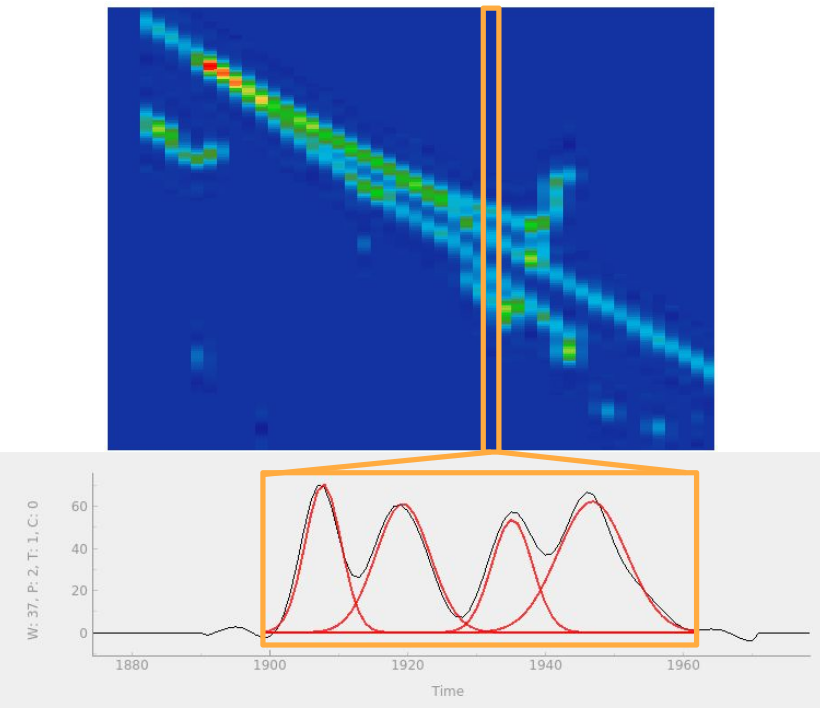
\includegraphics[width=0.5\textwidth]{gaushit}
\caption[Hit Finding Diagram]{
Diagram illustrating the hit finding algorithm on a single wire \cite{EdPhD}.
}
\label{fig:gaushit}
\end{figure}

\subsection{Pandora Pattern Recognition}
\label{sec:pandora}

%Pattern Recognition: Pandora
The output hits from the hit finding process are then used to perform 3D reconstruction, which is performed with the Pandora pattern recognition package \cite{pandora}.
The package was first developed for the International Linear Collider and later extended to other LArTPC experiments.
It is made up of over 100 individual algorithms, each performing a specific task along the reconstruction chain.
The output from Pandora represents an interaction, containing a hierarchy of particles starting with a neutrino parent at the interaction vertex.
This reconstructed object is referred to as a \textit{slice}.

The reconstruction begins with a workflow to reconstruct cosmic-like objects that leave long tracks inside the detector.
This workflow performs a 2D clustering on each wire plane independently, followed by 3D reconstruction under the assumption that all clusters are track-like.
Then, a cosmic rejection is performed to identify if a cluster is cosmic-like or neutrino-like.
The cosmic removal at this stage is deliberately cautious such that only very unambiguous cosmic muons in nature are removed.

The remaining clusters are then input into a second workflow dedicated towards neutrino reconstruction.
This workflow begins with a slicing algorithm that divides clusters into \textit{slices}, where each slice encapsulates hits coming from a single origin, representing an interaction.
Then, 2D clustering is re-performed on each wire plane independently, however, with a new assumption that clusters can be both track-like and shower-like.
A vertexing algorithm then identifies the interaction vertex of the slice and its associated clusters.
A series of pattern matching algorithms grows the interaction out of the neutrino vertex and performs 3D reconstruction by matching 2D clusters across different planes.
The output 3D reconstructed object associated with a vertex ideally represents a \textit{particle} produced from an interaction.

At this stage, a \textit{track score} is assigned to a particle if it has a track-like or a shower-like topology, which is determined by a dedicated Boosted Decision Tree (BDT).
The development work on the track-shower separation BDT and its importance not only in the reconstruction workflow but also in the analysis workflow will be covered in Sec. \ref{sec:trkshwbdt} next.
Both track and shower reconstruction tools are then performed on the particle. 
Finally, a hierarchy algorithm is performed to classify the hierarchy of particles in a slice, starting with a neutrino parent vertex, and other particles are children, grandchildren, etc. of the parent.                             

%Calorimetry reconstruction
The last stage of reconstruction is calorimetry computation for the output slices and their associated particles.
Both track and shower calorimetry computations first convert ADC units to charges, or the number of electrons, by multiplying by a charge calibration constant.
The track calorimetry then computes the energy from the charge using the ModBox recombination formalism, factoring in the electric field distortion (See Eq. \ref{eq:recomb_modbox}, Sec. \ref{sec:simDeltaRay}).
Meanwhile, the shower calorimetry reconstruction converts the measured charge to energy by multiplying it by a shower calibration constant, factoring in an averaged recombination factor. 
Once the SBND detector is operational, the calibration constants will be measured via dedicated calibration runs.
The charge calibration constant is expected to be computed from a sample of the anode-to-cathode crossing muons while the shower calibration constant can be acquired from using a standard candle of the neutral pion invariant mass \cite{uboone_gamma}.

\subsection{Track-Shower Separation Boosted Decision Tree}
\label{sec:trkshwbdt}

As previously discussed, reconstructed particles from Pandora are assigned a track score determined by BDT, which is a binary classification machine learning tool.
The track score spans between 0 and 1 such that if a particle has a very high track score close to 1, then the particle is track-like.
Otherwise, if the track score is very close to 0, then the particle is shower-like.

The track-shower BDT has become more important in the reconstruction as well as the analysis workflow due to a new reconstruction paradigm introduced by Pandora.                                      
The traditional reconstruction approach was to perform only either track or shower reconstruction on a particle based on its track score.
The new paradigm performs both track and shower reconstruction on a particle regardless of the track score.
All reconstructed particles now have two sets of reconstruction variables for track-like and shower-like.
The users have the freedom to decide which variables to use depending on their signal topology, and thus not pre-determined by Pandora.
The track score can inform which appropriate reconstruction variables should be used for the analysis. 

The track-shower separation BDT was trained on a series of reconstruction variables and was updated to include new variables in the training.
The original BDT includes variables describing the geometrical topology of the particle such as its length, distance and direction with respect to the parent vertex, as well as calorimetry variables describing the charge distribution of the particle.
More details of the input variables and the training of the BDT can be found in Ref. \cite{EdPhD}.
The update extended beyond the original work to include a brand new set of variables describing how cone-like the charge distribution of a particle as well as a new variable describing the particle hierarchy.

The cone variables were first developed by M. Haigh for particle identification \cite{warwick_pid} and were imported into Pandora for reconstruction purposes.
There are three variables: (1) halo-total ratio, (2) concentration and (3) conicalness as depicted in Fig. \ref{fig:cone_variables}.
The diagrams depict the hit distribution of a particle, where each circle represents a hit associated with a charge value and the star represents the vertex of the hit cluster.
The illustration is in 2D for simplicity, however the variables are computed in 3D.
The first variable is the halo-total ratio, illustrated in Fig. \ref{fig:halototalratio}.
The region outside of the Moliere radius, defined such that 90\% of the cluster energy is contained within this radius, is considered the halo region.
The hits in the halo are shown as green circles whereas any other hits are shown as grey circles.
The halo-total ratio is then defined as 
\begin{equation}
	Halo\ - Total\ Ratio = \frac{Charges\ in\ The\ Halo}{Total\ Charges}
\end{equation}

\begin{figure}[b!]
        \centering
        \begin{subfigure}[b]{0.495\textwidth}
            \centering
            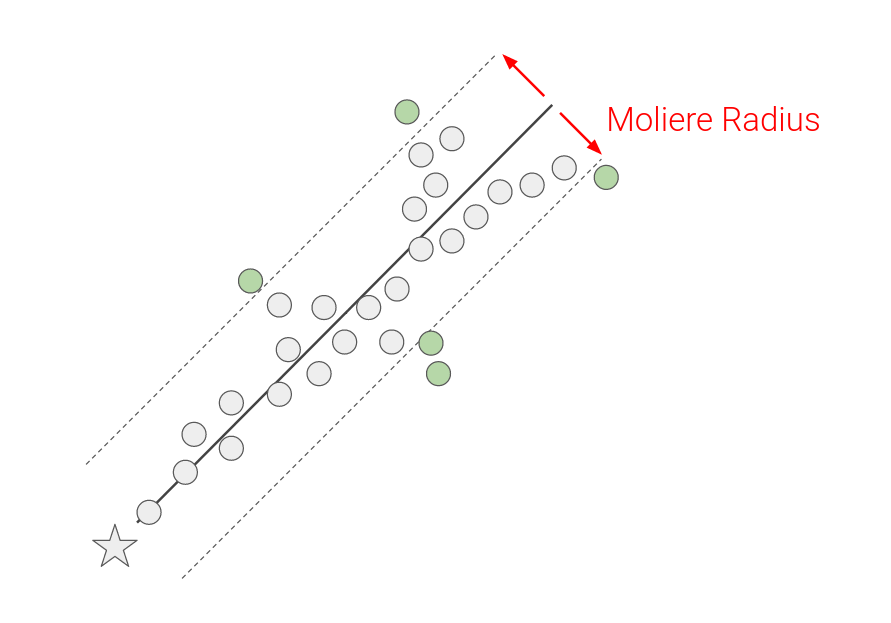
\includegraphics[width=\textwidth]{HaloTotalRatio}
            \caption{Halo-Total Ratio}%
            \label{fig:halototalratio}
        \end{subfigure}
        \hfill
        \begin{subfigure}[b]{0.495\textwidth}  
            \centering 
            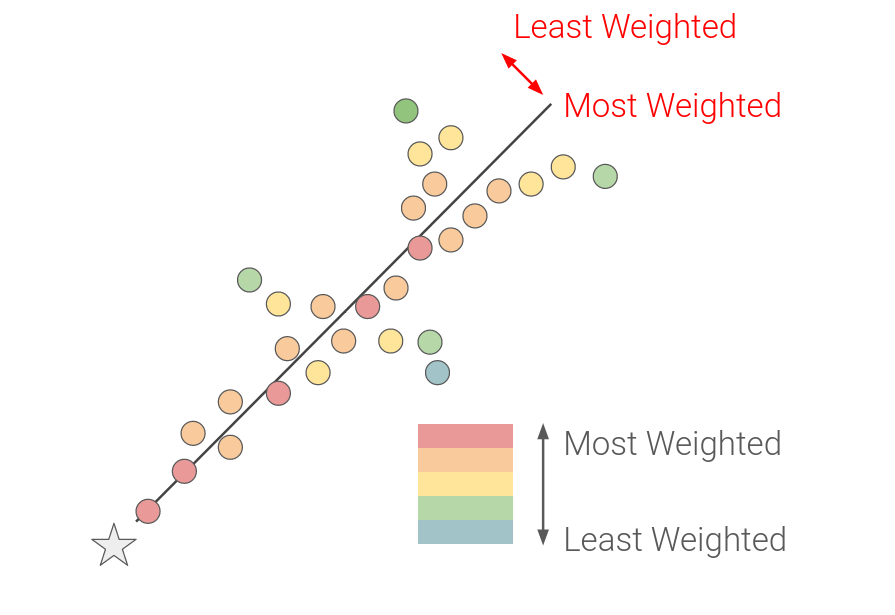
\includegraphics[width=\textwidth]{Concentration}
            \caption{Concentration}%
            \label{fig:concentration}
        \end{subfigure}
        \hfill
        \begin{subfigure}[b]{0.495\textwidth}  
            \centering 
            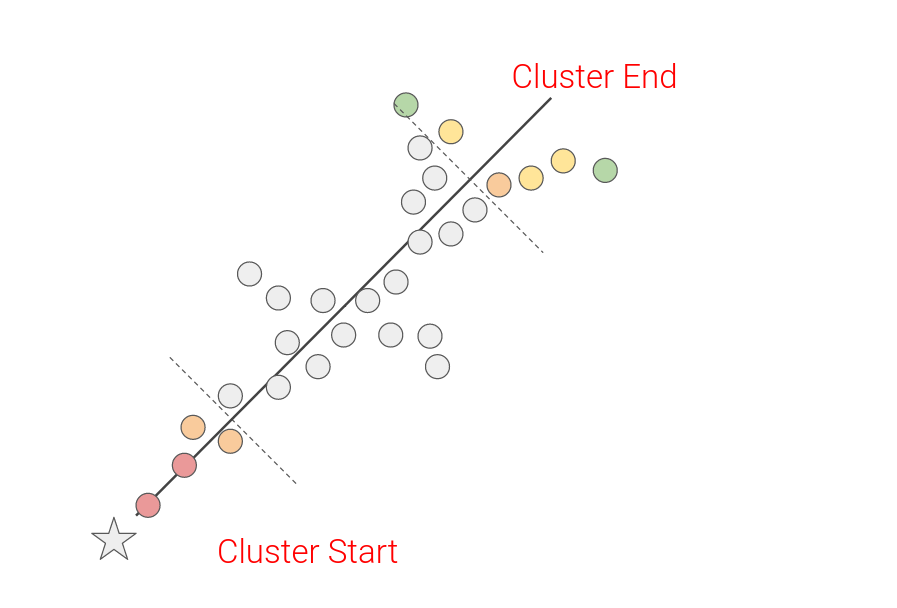
\includegraphics[width=\textwidth]{Conicalness}
            \caption{Conicalness}%
            \label{fig:conicalness}
        \end{subfigure}
        \caption[Cone-Like Variable Diagrams]{
	Diagrams illustrating the variables describing how cone-like the charge distribution of a particle .
	}
        \label{fig:cone_variables}
\end{figure}

The second variable is called concentration, accounting for how concentrated the charge distribution is to the centre of the cluster.
This is depicted in Fig. \ref{fig:concentration}, where each hit is assigned a colour showing how weighted it is with respect to its orthogonal distance to the cluster direction.
The closer the hit to the centre, the more weighted it is.
The concentration variable is defined as the total weighted charges divided by the total charge as following
\begin{equation}
	Concentration = \frac{\sum Charge \times Weight}{Total\ Charges}
\end{equation}
Finally, the conicalness variable examines the hit distribution at the end and the start of the cluster as depicted in Fig. \ref{fig:conicalness}. 
It is defined as the ratio between the concentration at the end of the cluster compared to at the start of the cluster
\begin{equation}
	Conincalness = \frac{Concentration\ at\ The\ End}{Concentration\ at\ The\ Start}
\end{equation}

On top of the cone variables, another new variable was introduced to the track-shower separation BDT to describe the hierarchy of the particle within the reconstructed interaction or slice.
For a given particle, the daughters originating from that particle are identified and their number of hits are counted.
The distributions of the four new variables for a track-like and shower-like particle are shown in Fig. \ref{fig:bdt_features}.
The concentration and conicalness variables display the strongest separation power between tracks and showers compared to the halo-total ratio and the number of daughter hits variables.

\begin{figure}[b!]
        \centering
        \begin{subfigure}[b]{0.45\textwidth}
            \centering
            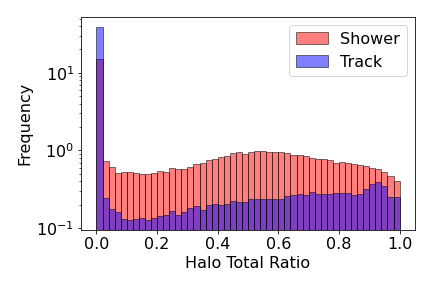
\includegraphics[width=\textwidth]{Feature_Halo_Total_Ratio}
            \caption{}%
        \end{subfigure}
        \hfill
        \begin{subfigure}[b]{0.45\textwidth}  
            \centering 
            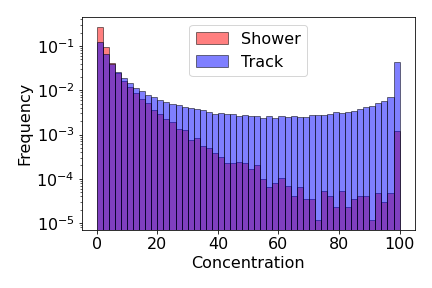
\includegraphics[width=\textwidth]{Feature_Concentration}
            \caption{}%
        \end{subfigure}
        \hfill
        \begin{subfigure}[b]{0.45\textwidth}  
            \centering 
            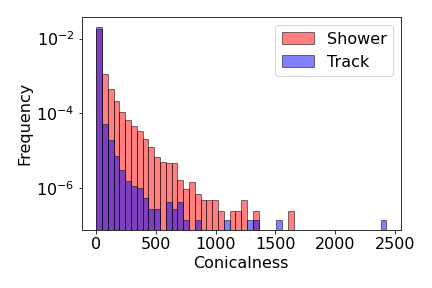
\includegraphics[width=\textwidth]{Feature_Conicalness}
            \caption{}%
        \end{subfigure}
        \hfill
        \begin{subfigure}[b]{0.45\textwidth}  
            \centering 
            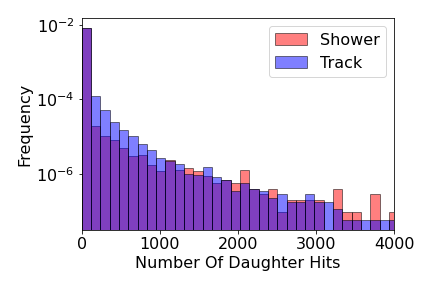
\includegraphics[width=\textwidth]{Feature_Number_Of_Daughter_Hits}
            \caption{}%
        \end{subfigure}
        \caption[New Variable Distributions of Track-Shower Separation BDT]{
	Distributions of new variables for the track-shower BDT: (a) halo-total ratio, (b) concentration, (c) conicalness and (d) number of daughter hits.
	}
        \label{fig:bdt_features}
\end{figure}

Fig. \ref{fig:bdt_score} shows the score distribution of the BDT retrained with the four new variables.
The left figure shows two distinct distributions in red and blue for showers and tracks respectively.
This demonstrates a good separation power of the BDT, where particles with a score less than 0.5 closely resemble showers whilst particles with a score more than 0.5 are more track-like.
The score distribution is broken down into different particle types as shown in the right figure.
The distribution is expected given that electrons and photons leave electromagnetic shower activities inside the detector whilst charged particles like muons, pions and protons leave track-like signatures. 
The updated BDT resulted in $0.1\sim2.0\%$ improvement in correctly classifying particle type as shower-like or track-like.
The track-shower separation score distribution will be used in downstream high level analysis tools, to be detailed in Sec. \ref{sec:subsystem_match}, as well as will be employed as a cut variable in the HNL selection, to be detailed in Chapter \ref{ChapterSelect}.

\begin{figure}[htbp!]
        \centering
        \begin{subfigure}[b]{0.495\textwidth}
            \centering
            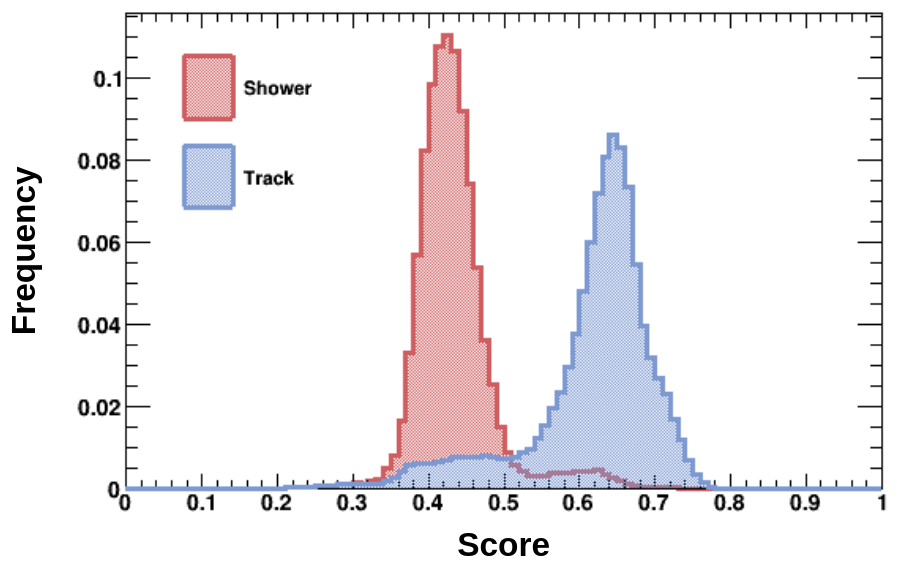
\includegraphics[width=\textwidth]{bdt_score_trk_shw}
            \caption{}%
        \end{subfigure}
        \hfill
        \begin{subfigure}[b]{0.495\textwidth}  
            \centering 
            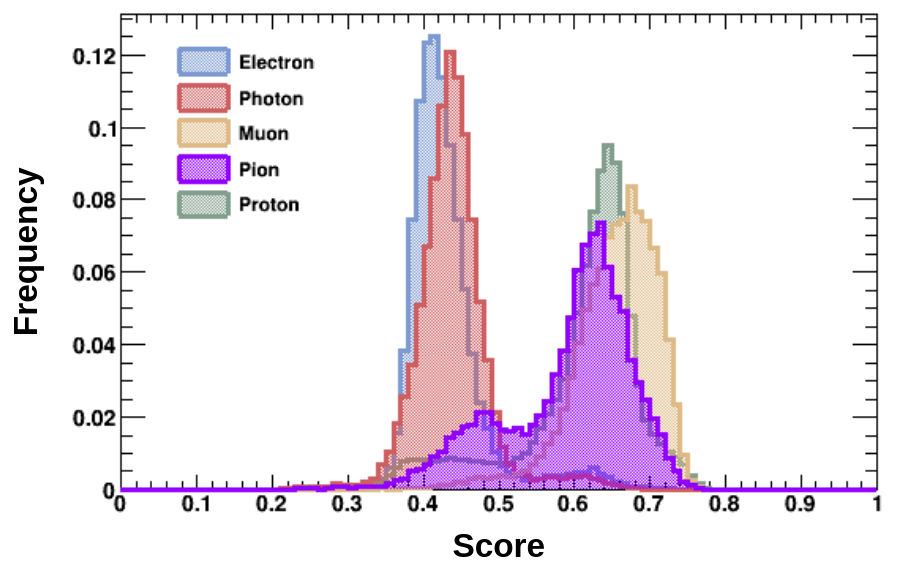
\includegraphics[width=\textwidth]{bdt_score_particle}
            \caption{}%
        \end{subfigure}
        \caption[Score Distributions of Updated Track-Shower Separation BDT]{
	Score distribution of the updated track-shower BDT, plotted for (a) track-like and shower-like particles and (b) different particle types.
	}
        \label{fig:bdt_score}
\end{figure}

\section{Photon Detection System and Cosmic Ray Tagger Reconstruction}
\label{sec:reco_others}

The reconstruction workflow of the two detection subsystems, PDS and CRT, are detailed in the following Sec. \ref{sec:reco_pds} and \ref{sec:crt_reco}. 

\subsection{Photon Detection System Reconstruction}
\label{sec:reco_pds}

The reconstruction of optical detectors, PMTs and X-ARAPUCAs, share the same steps of waveform deconvolution, hit finding and light reconstruction.
However, different algorithms and parameter settings are required for each optical detector type due to their different responses.
More details on the PDS reconstruction at the SBND detector can be found in Ref. \cite{sbnd_pds_paper}.
Here focuses on the reconstruction of PMT waveforms, which have an averaged Single Electron Response (SER) pulse peaking at $\sim 25$ ADC and a full width at half maximum of $\sim$ 10 ns.
The fast response of PMT plays a key role in the nanosecond timing resolution requirement for the HNL search.

The first step is the PMT waveform deconvolution, aiming mainly at noise removal.% and baseline determination.
Fig. \ref{fig:pds_reco_deconvolution} depicts an example of a simulated PMT waveform before and after the deconvolution.
The top figure shows the number of \textit{true}, or MC, PhotoElectrons (PEs) seen by a PMT as a function of time in green.
The middle figure shows the raw waveform resulting from the deposited PEs in blue, convolved with the PMT response and noise.
The AC circuits of PMTs lead to over/undershoot features across the raw waveform with respect to the baseline.
A 1D deconvolution and a high frequency Gaussian filter are applied subsequently.
The deconvolved waveform is shown in orange in the bottom figure, demonstrating that bipolarity features are removed while maintaining peaks' magnitudes and positions.

\begin{figure}[b!]
        \centering
        \begin{subfigure}[b]{0.59\textwidth}
            \centering
            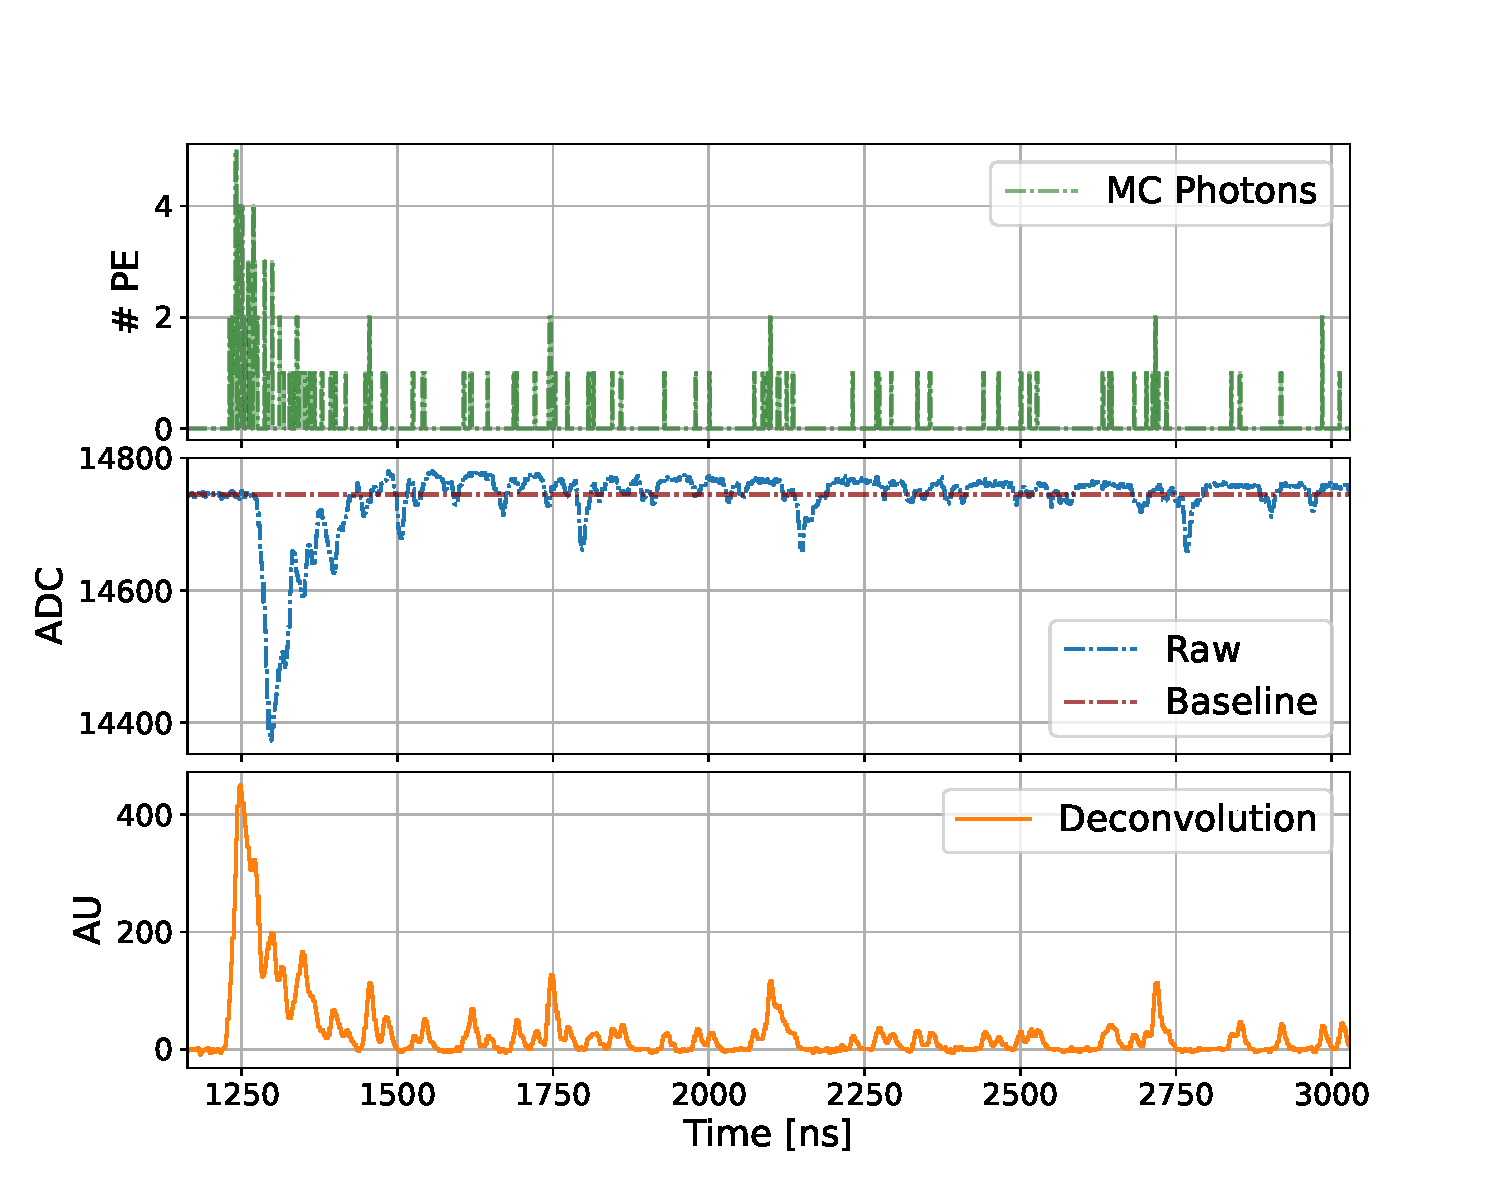
\includegraphics[width=\textwidth]{pds_reco_deconvolution}
            \caption{Waveform Deconvolution}
            \label{fig:pds_reco_deconvolution}
        \end{subfigure}
        \hfill
        \begin{subfigure}[b]{0.4\textwidth}  
            \centering 
            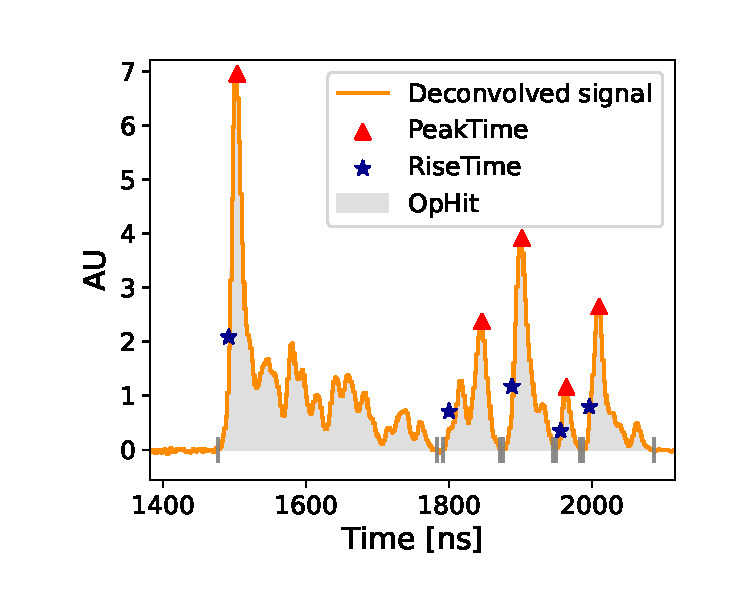
\includegraphics[width=\textwidth]{pds_reco_hit_finding}
            \caption{Hit Finding}
            \label{fig:pds_reco_hit_finding}
        \end{subfigure}
        \caption[Waveform Deconvolution and Hit Finding on PMT Waveforms]{
	Example demonstrating the waveform deconvolution and hit finding applied to a PMT waveform \cite{sbnd_pds_paper}.
	}
        \label{fig:pds_reco}
\end{figure}

Hit finding is performed next on deconvolved PMT waveforms, beginning with a baseline subtraction.
Optical hits are identified by finding pulses that go above a threshold of $1/4$ the amplitude of the deconvolved SER and 3 standard deviations away from the baseline root mean square.
Fig. \ref{fig:pds_reco_hit_finding} demonstrates a PMT wavefrom after baseline subtraction with 4 identified optical hits.
Peak times, corresponding to the maximum of an optical hit, are denoted with red triangles.
The first optical hit contains multiple peaks merged into a single optical hit due to multiple photons arriving very closely in time to the PMT.
The rise time of an optical hit is defined as when the first peak goes above 15\% of its amplitude, denoted with blue stars.
It is an estimation of the arrival time of the first photon contributing to the optical hit. 
The integral of the optical hit is used to compute the number of PEs.
%which is calculated using a 400 ns portion at the start and end of the deconvolved waveform, resulting in the waveform shown in orange.
%This results in a resolution of 1.6 ns in estimating the arrival time of the first photon contributing to the optical hit.

Next, the light reconstruction algorithm then clusters optical hits into an \textit{optical flash}.                                                                                            
The length of an optical flash is set as 8 $\mu$s to account for the total light produced in a neutrino interaction, from both prompt and slow components of scintillation photons.
The clustering algorithm is based on the number of PEs of optical hits, timing distribution between hits and geometrical location of the PMTs.                                                  
The number of PEs in an optical flash is the sum of PEs of optical hits clustered in that flash, representing the total light generated by an interaction. 

The start time of the optical flash represents the start time of an interaction, $t_0$, which is the key variable of the HNL search, and therefore requires great care in reconstruction.
The flash start time is the average of the rise time of optical hits in a flash, only considering PMTs that contribute 50\% of the prompt light in the 30 ns window of the largest PE pulse.
Then, a correction is applied for the propagation of the photons from the scintillation position in the TPC to the PMTs.

\begin{figure}[b!]
\centering    
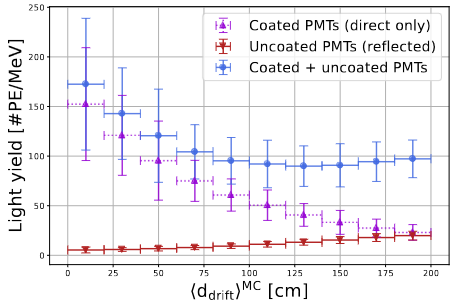
\includegraphics[width=0.55\textwidth]{light_yield_sim}
\caption[Reconstructed Light Yield at SBND]{
Reconstructed light yield as a function of the mean drift distance \cite{sbnd_pds_paper}. 
}
\label{fig:light_yield_Diego}
\end{figure}

The correction can be computed by exploiting the high density of PMTs as well as having coated and uncoated PMTs sensitive to direct VUV light and reflected visible light respectively.
Fig. \ref{fig:light_yield_Diego} shows the reconstructed light yield seen by TPB-coated and uncoated PMTs based on simulation, as a function of the photon mean drift distance, $d_{drift}$ ($x$-axis).
The error bars show the uncertainty due to the geometrical effects of the detector.
Closer to the anode at $d_{drift} = 0 $ cm, the light yield primarily comes from direct VUV photons, detected by coated PMTs as shown in purple.
Closer to the cathode at $d_{drift} = 200 $ cm, and hence the reflective foils, the contribution to the light yield from reflected visible photons increases, which are detected by uncoated PMTs as shown in red.
For a given scintillation position, and therefore a drift position, the amount of direct and visible photons leads to a specific ratio of the two components seen by PMTs.
This ratio is used to compute the correction for the drift propagation effect when reconstructing the flash time.                                                                              
The timing resolution of the flash time varies by $\sim 2$ ns across the entire drift distance, demonstrating the excellent capability of the PDS reconstruction at SBND \cite{sbnd_pds_paper}.

\subsection{Cosmic Ray Tagger Reconstruction}
\label{sec:crt_reco}

The reconstruction of the CRT subsystem is the simplest compared to the TPC and the PDS.
As previously detailed, the output data of the CRT readouts are in a group of 32 ADC values, for a single ADC per SiPM.
The reconstruction begins with a hit finding algorithm to identify which pair of SiPMs in the group goes above a threshold.
The SiPM pair determines the lateral position of a cosmic muon hit within a CRT strip.
A clustering algorithm groups hits from orthogonal CRT strips of the same wall within a 50 ns window to yield 3D space points.
For each CRT space point, the timing and calorimetry information is calculated and corrected for the propagation effect from the hit position to the SiPM.
CRT space points from multiple CRT walls are matched together to form a CRT track based on the goodness of timing agreement and prioritising three-point tracks over two-point tracks.
The outputs of the CRT reconstruction are both CRT space points and CRT tracks. 
%The final step is to match space points from multiple CRT walls to form a CRT track.
%Candidate tracks are evaluated from any combinations of space points from different walls within a 100 ns coincidence window.
%The best track candidate is selected by the goodness of timing agreement and prioritising three-point tracks over two-point tracks. 

%********************************** %First Section  **************************************
\section{High Level Analysis Tools}
\label{sec:reco_ana_tools}

The reconstructed variables from each detection subsystem, slices from the TPC, flashes from the PDS, space points and tracks from the CRTs, can be used collectively by downstream algorithms to compute useful characteristics regarding the interaction.
This section covers the main high level analysis tools used in the HNL search and their usage will be detailed in Chapter \ref{ChapterSelect}.
Firstly, Sec. \ref{sec:subsystem_match} provides the details on how variables from different detection subsystems can be matched to the same interaction.
Presented in Sec. \ref{sec:crumbs} are the cosmic rejection tool.
Finally, Sec. \ref{sec:razzled} illustrates the method employed for particle identification.

\subsection{Subsystem Matching}
\label{sec:subsystem_match}

The reconstructed tracks using the TPC can be matched to a space point or tracks from the CRTs to provide additional information for cosmic rejection.
An example is that a through-going cosmic ray produces a long track in the TPC as well as deposit energy in the nearest CRT walls where the track starts and ends. 
Another example is that tracks produced in the TPC deposit energy in the nearest CRT strips only when they enter or exit the detector, enabling the tagging of stopping cosmic muons or exiting neutrinos.

Two types of matching are performed: (1) matching a TPC track to CRT space points and (2) matching a TPC track to CRT tracks.
The former method extrapolates the TPC track and matches with the nearest CRT space points by computing a Distance of Closest Approach (DCA), confining the matching to a single CRT wall. 
The latter method uses a compound score from the average DCA of a TPC track to many CRT tracks and the angle between them, enabling matching a TPC track to many CRT walls.
Both methods use the timing information of the CRT objects for further constraints and no matching duplications are allowed.

The second subsystem matching of interest is matching an interaction reconstructed using TPC wires, a slice, to an interaction reconstructed using PMTs, a flash.                                        
This matching is vitally important since the flash time matched to a slice represents the start time of the interaction reconstructed in that slice.
It is the key variable employed to separate the HNL signal from the SM neutrino background, which will be detailed in Chapter \ref{ChapterSelect}.

The matching of the TPC to the PDS is done with the \texttt{Opt0Finder} module \cite{opt0finder_module}.
The matching is based on the estimation of charge yield in a slice seen by the wires to predict the light yield, and whether the predicted light yield is in good agreement with the measured light yield seen by PMTs.
Firstly, the charge yield of a slice is converted to energy to light yield based on the topology of particles in the slice.
The track score of the particles in the slice, assigned by the track-shower separation BDT detailed in Sec. \ref{sec:trkshwbdt}, is used to indicate whether the particle is track-like or shower-like.
If the particle is track-like, the calorimetry computation uses the ModBox recombination formalism with the charge-light anti-correlation. 
If the particle is shower-like, the calorimetry computation uses a charge-to-light conversion by multiplying a constant.     

From the estimated light yield, a hypothesis of the number of PE seen by each PMT is constructed by re-running the semi-analytical light library.
Finally, the hypothesis PE is compared to the measured PE for any given flash by a $\chi^2$ computation.
The flash that is best matched to a slice is the one with the lowest $\chi^2$.
Only one-to-one match is allowed such that only a single optical flash is matched to a slice.

A useful variable from this matching process is the comparison between the hypothesis PE predicted from the measured charge, denoted as $L_{\mathrm{Q}}$, and the measured PE seen by PMTs, denoted as $L$.                                                                            
The variable is defined as follows
\begin{equation}
\label{eq:opt0fraction}
        \frac{L_{\mathrm{Q}} - L}{L}
\end{equation}
This fraction indicates the level of agreement between $L_{\mathrm{Q}}$ and $L$, and thus, the level of agreement of the interaction calorimetry using the measured charge or the measured light.
If the fraction is positive, the predicted light from the measured charge is overpredicted compared to the measured light, otherwise, it is underestimated.
This variable is particularly useful in the selection of HNL signals, which will be further elaborated in Chapter \ref{ChapterSelect}.

\subsection{Cosmic Rejection}
\label{sec:crumbs}

Cosmic Rejection Using a Multi-system Boosted decision tree Score (CRUMBS) uses all three detection subsystems of SBND for cosmic rejection \cite{crumbs}. 
CRUMBS is a binary classification BDT that outputs a score whether a reconstructed slice is cosmic-like or neutrino-like.
Reconstruction variables from all three detection subsystems that are complementary to each other are input into CRUMBS, and therefore vastly reduce inefficiencies compared to using a single system.
The TPC information includes variables describing a particle as both neutrino-like and cosmic-like, accounting for its charge distribution, position within the TPC and calorimetry.  
The PDS information is from the flash best matched to the slice of interest, particularly the number of PEs in the flash and the $\chi^{2}$  from the matching agreement.                        
Finally, the CRT information consists of both TPC-CRT matching algorithms, including the timing information of the CRT space points/tracks and the matching score.
The score distribution of CRUMBS shows a significant separating power between neutrino-like signals and cosmic-like backgrounds.
%CRUMBS was trained using the TMVA toolkit \cite{tmva} on MC samples of neutrinos, evenly distributed between $CC\nu_{\mu}$ and $CC\nu_{e}$, and cosmic muons.

\subsection{Particle Identification}
\label{sec:razzled}

The main particle identification tool at SBND is called Razzled \cite{razzled}, which is a multi-classification BDT designed to identify particle type that would deposit energy inside SBND: $e$, $\gamma$, $\mu$, $\pi$ and $p$.
The reconstruction variables input into Razzled are only TPC variables, mainly from the Pandora package.
There are three categories of variables for training Razzled: (1) generic reconstruction variables, (2) track-like variables and (3) shower-like variables.
The generic variables describe the particle multiplicity, topology, directionality and charge distribution.
Track reconstruction variables include track lengths, calorimetry, kinematics in the stopping region to identify Bragg peak, and multiple coulomb scattering for $\mu$-$\pi$ separation.
Shower reconstruction variables include shower conversion gaps, opening angles and calorimetry aiming towards $\gamma$-$e$ separation.
A full description of the input variables and training can be found in Ref. \cite{EdPhD}.
This collection of variables allows Razzled to exploit the correlation between variables, thereby significantly improving the identification performance over traditional hand cuts.
For each reconstructed particle, Razzled outputs a score for each particle type and assigns the highest particle type score to that particle.

\section{Concluding Remarks}
\label{sec:reco_concluding_remarks}

The overall reconstruction workflow of SBND has been described, outlining the reconstruction process for each detection system, the TPC, the PDS and the CRT.
The three detection subsystems together provide complementary information regarding the underlying reconstructed interaction and have been used collectively by different analysis tools for different purposes.
Focusing on the HNL search, the background rejection and signal selection will be based on a combination of variables and tools employing all three subsystems to achieve a high signal-to-background ratio, as will be discussed in Chapter \ref{ChapterSelect}.

Particularly, the most important variable is the reconstructed interaction time, $t_0$, which is subsequently used to compute the arrival time at the front face of SBND.
These timing variables, having a resolution of $\sim$ 2 ns, enable the reconstruction Gaussian-shaped neutrino beam bucket and therefore, are powerful discriminations to differentiate HNLs from SM neutrinos.
To achieve such high timing resolution at the high level reconstruction, the low level readout electronics must have sufficient timing resolution to maintain a high quality data stream at a high sampling rate.
The timing characterisation of the readout electronics will be discussed in Chapter \ref{ChapterDAQ} next.

%The event building process of the DAQ relies on the timing information acquired from each subsystem. 
%This process assembles the foundation of physics event upon which low level and high level reconstructions are built to achieve nanosecond timing resolution.
